\documentclass[11pt]{article}

\usepackage[letterpaper,top=0.72in,bottom=0.82in,left=0.9in,right=0.9in]{geometry}
\usepackage[T1]{fontenc}
\usepackage{newtxtext,newtxmath}
\usepackage{microtype}
\usepackage{booktabs}
\usepackage{array}
\usepackage{tabularx}
\usepackage{graphicx}
\usepackage{xcolor}
\usepackage{enumitem}
\usepackage{titlesec}
\usepackage[hidelinks]{hyperref}

\definecolor{navy}{HTML}{19324D}
\definecolor{blue}{HTML}{315B7D}
\definecolor{lightblue}{HTML}{EDF4F8}
\definecolor{linegray}{HTML}{B8C2CC}

\hypersetup{
  colorlinks=true,
  linkcolor=navy,
  citecolor=navy,
  urlcolor=blue,
  pdftitle={Aggregate and Malware-Family Calibration in the Released EMBER2024 Detector},
  pdfauthor={Tara Dixit}
}

\titleformat{\section}{\large\bfseries}{\thesection}{0.55em}{}
\titleformat{\subsection}{\normalsize\bfseries}{\thesubsection}{0.55em}{}
\titlespacing*{\section}{0pt}{1em}{0.35em}
\titlespacing*{\subsection}{0pt}{0.8em}{0.25em}

\setlength{\parindent}{1em}
\setlength{\parskip}{0.12em}
\setlist[itemize]{leftmargin=1.3em,itemsep=0.15em,topsep=0.25em}
\clubpenalty=10000
\widowpenalty=10000
\displaywidowpenalty=10000
\brokenpenalty=10000
\hyphenpenalty=5000
\exhyphenpenalty=5000

\pagestyle{plain}

\makeatletter
\setlength{\@fptop}{0pt}
\setlength{\@fpsep}{14pt}
\makeatother

\newcommand{\code}[1]{\texttt{#1}}

\begin{document}

\begin{center}
  \rule{\textwidth}{2.2pt}
  \vspace{0.18cm}

  {\Large\bfseries Aggregate and Malware-Family Calibration in the Released EMBER2024 Detector\par}

  \vspace{0.2cm}
  \rule{\textwidth}{0.7pt}
  \vspace{0.42cm}

  {\normalsize\bfseries Tara Dixit\par}
  \vspace{0.06cm}
  {\small Stanford University\par}
  {\small Stanford, CA\par}
  {\small\href{mailto:tdixit@stanford.edu}{\texttt{tdixit@stanford.edu}}\par}
\end{center}

\vspace{0.2cm}

\begin{center}
\begin{minipage}{0.78\textwidth}
\begin{abstract}
\small
The released EMBER2024 PE detector has strong overall scores, but aggregate
metrics may hide errors for specific malware families. I evaluated the released
LightGBM model on 540,000 PE records represented by 2,568 \code{thrember}
features. The data contain 360,000 Win32, 120,000 Win64, and 60,000 Dot\_Net
records. The released archives contained duplicated structural halves, so the
evaluation kept the first documented half of each weekly member. The selected
data have 539,940 unique hashes. Sixty hashes occur twice across member and week
boundaries, with no label, family, file-type, or detector-input conflicts. The
model reaches 0.9803222222 accuracy, 0.9981880554 ROC AUC, a 0.0147949965 Brier
score, 0.0030850838 expected calibration error (ECE), and 0.0277246070 maximum
calibration error (MCE) with 15 bins. These aggregate values are strong. Family
results are different. Among families with at least 100 malicious records,
\code{malicord} has a false-negative rate of 0.851852 and ECE of 0.602358.
\code{lazzzy} and \code{rugmi} also have false-negative rates above 0.61. The
family results are descriptive, not causal. They show that good aggregate
calibration can coexist with large errors in smaller groups.
\end{abstract}
\end{minipage}
\end{center}

\section{Introduction}

EMBER2024 is a malware benchmark with data from several file types and time
periods \cite{joyce2025ember}. Its released PE detector is a LightGBM model
\cite{ke2017lightgbm}. This study asks a narrow question:

\begin{quote}
\itshape Can strong aggregate calibration hide high-confidence false negatives
for specific malware families in the released EMBER2024 PE detector?
\end{quote}

Calibration describes whether a model's stated confidence matches its observed
accuracy. A model can be well calibrated on average while giving poor results
for a subgroup. This matters in malware detection because families differ in
size, behavior, and representation in the data.

I evaluate the released model without retraining it. I report aggregate
accuracy, ROC AUC, Brier score, ECE, and MCE. I then measure false-negative rate
and ECE within malicious families. The main result is simple: the aggregate
scores are strong, but several families have high false-negative rates and
large calibration gaps.

\section{Data}

\subsection{Released PE test records}

The evaluation uses the PE part of EMBER2024. Table~\ref{tab:data} shows the
documented test counts. The 12 test weeks contain equal numbers of malicious
and benign records overall.

\begin{table}[!htbp]
\centering
\caption{Evaluated PE records.}
\label{tab:data}
\begin{tabular}{lrr}
\toprule
File type & Records per week & Total records \\
\midrule
Win32 & 30,000 & 360,000 \\
Win64 & 10,000 & 120,000 \\
Dot\_Net & 5,000 & 60,000 \\
\midrule
Total & 45,000 & 540,000 \\
\bottomrule
\end{tabular}
\end{table}

The three compressed source archives total 3,990,366,412 bytes. Controlled
extraction produced 36 JSONL members totaling 17,655,416,292 bytes. Each weekly
member contained two ordered structural halves. Corresponding rows matched on
SHA-256, label, family, file type, week, and all 12 inputs used by the PE
feature extractor. Only the \code{caps}, \code{mbc}, and \code{ttps} fields
differed. Those fields are not detector inputs.

The selection keeps the first documented half of each member: 30,000 Win32,
10,000 Win64, or 5,000 Dot\_Net rows. This is a fixed structural rule. It does
not claim that the first half is better. The result has 539,940 unique hashes.
Of these, 539,880 occur once and 60 occur twice across member and week
boundaries. The repeated rows have no label, family, file-type, or
detector-input conflicts.

\subsection{Prepared inputs}

The official \code{thrember} PE extractor produces 2,568 features per record.
The released LightGBM model also reports 2,568 input features. Preparation
preserved selection order and produced a \code{float32} feature matrix, an
\code{int32} label vector, and aligned metadata. Inference produced one finite
\code{float64} malicious-class probability per row.

\section{Method}

\subsection{Aggregate measures}

Predictions at or above 0.5 are malicious. Accuracy uses that threshold. ROC
AUC measures ranking over both classes. The Brier score is the mean squared
difference between a probability and its binary label \cite{brier1950}.

ECE and MCE follow common fixed-bin summaries \cite{guo2017calibration}. For a
probability $p$, predicted-label confidence is the larger of $p$ and $1-p$.
Confidence is divided
into equal-width bins over $[0.5,1.0]$. A bin gap is the absolute difference
between its mean confidence and accuracy. ECE is the count-weighted mean gap.
MCE is the largest nonempty-bin gap. The primary result uses 15 bins. Empty bins
have zero count, add no weight to ECE, and are omitted from MCE.

\subsection{Family measures}

Family analysis uses malicious records only. A prediction below 0.5 is a false
negative, so family false-negative rate equals one minus family accuracy. The
primary table includes families with at least 100 malicious records. It excludes
missing, blank, \code{unknown}, \code{none}, and \code{nan} family values
without changing the remaining labels. Family ECE uses the same 15-bin
predicted-label-confidence definition as the aggregate result.

The family estimates describe this dataset and model. They do not show that a
family name caused an error. The minimum count limits the noisiest small groups,
but it does not make every estimate stable.

\section{Results}

\subsection{Aggregate results}

Table~\ref{tab:aggregate} reports the verified results. The model is accurate
and ranks malicious records well. The Brier score, ECE, and MCE are also low.

\begin{table}[!htbp]
\centering
\caption{Aggregate results on 540,000 PE records.}
\label{tab:aggregate}
\begin{tabular}{lr}
\toprule
Metric & Value \\
\midrule
Accuracy & 0.9803222222 \\
ROC AUC & 0.9981880554 \\
Brier score & 0.0147949965 \\
15-bin ECE & 0.0030850838 \\
15-bin MCE & 0.0277246070 \\
\bottomrule
\end{tabular}
\end{table}

Figure~\ref{fig:reliability} compares confidence and observed accuracy. Most of
the mass is in the highest-confidence bins. The plotted points remain near the
diagonal at the aggregate level.

\begin{figure}[!htbp]
\centering
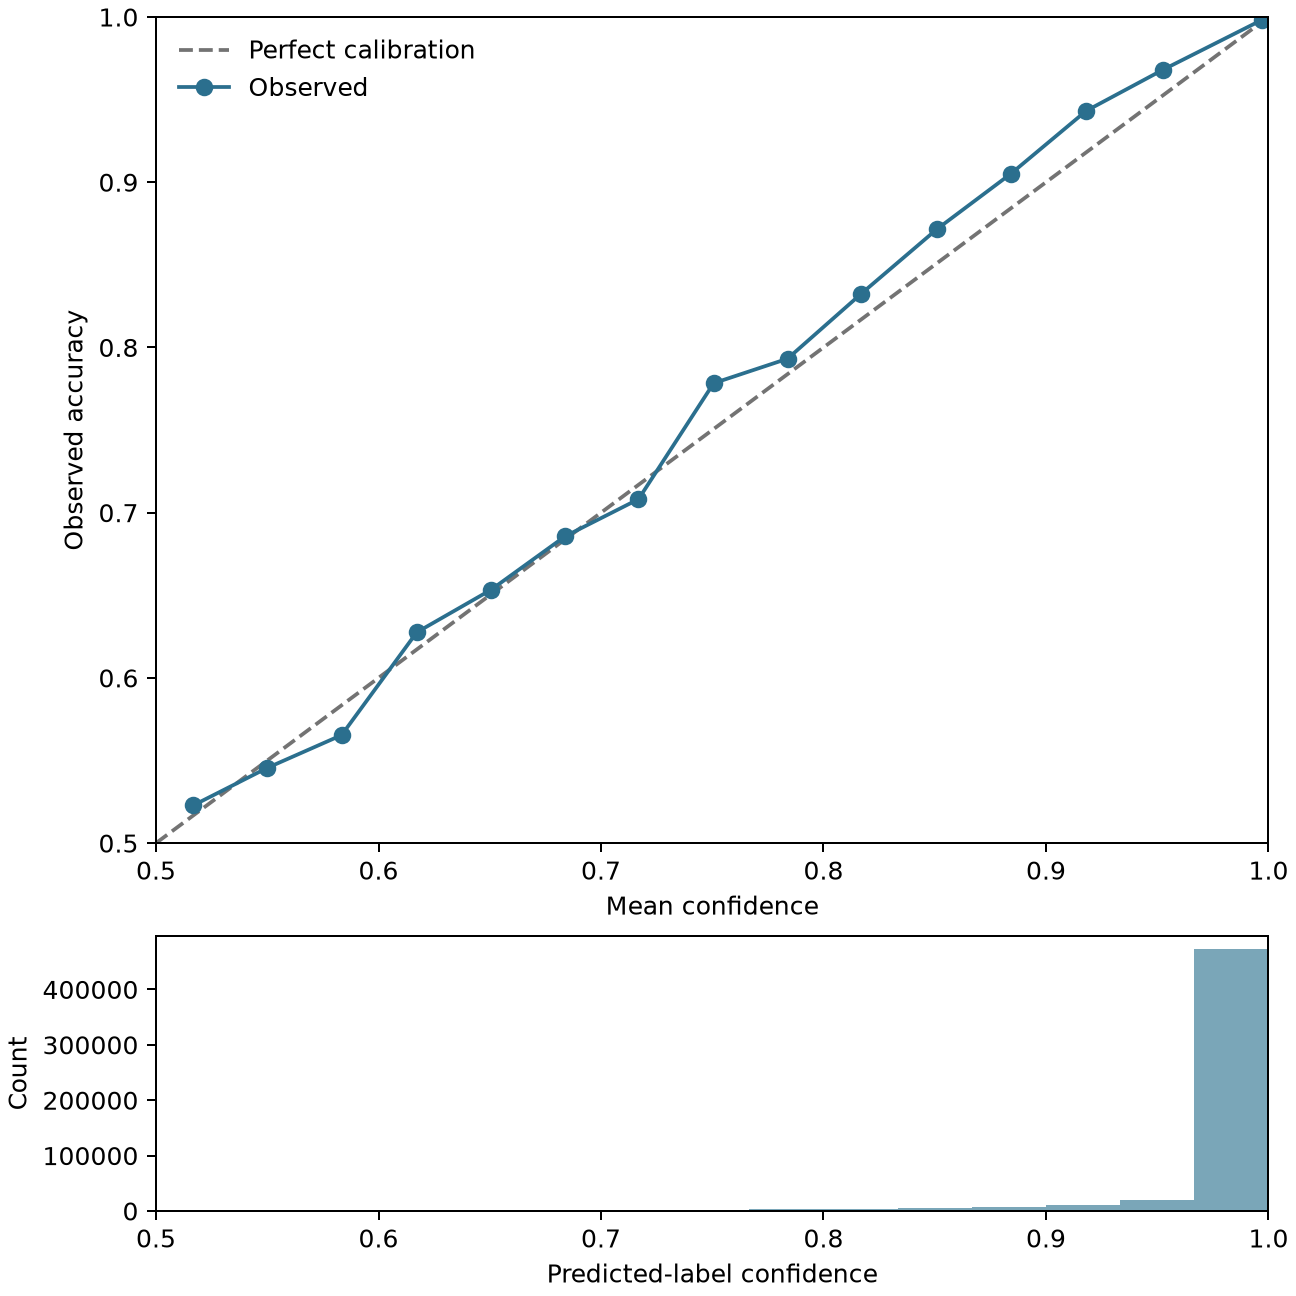
\includegraphics[width=0.68\textwidth]{../results/reliability_diagram.png}
\caption{Aggregate reliability diagram with 15 equal-width confidence bins.}
\label{fig:reliability}
\end{figure}

\subsection{Malware-family results}

The family results give a different view. Table~\ref{tab:families} lists six
families with large false-negative rates. \code{malicord} has 138 false
negatives among 162 malicious records. Its false-negative rate is 0.851852 and
its ECE is 0.602358. \code{lazzzy} and \code{rugmi} also have false-negative
rates above 0.61.

\begin{table}[!htbp]
\centering
\caption{Selected family results at the 100-record minimum.}
\label{tab:families}
\begin{tabular}{lrrr}
\toprule
Family & Malicious records & False-negative rate & 15-bin ECE \\
\midrule
\code{malicord} & 162 & 0.851852 & 0.602358 \\
\code{lazzzy} & 179 & 0.620112 & 0.452050 \\
\code{rugmi} & 256 & 0.617188 & 0.447200 \\
\code{goblin} & 165 & 0.406061 & 0.230170 \\
\code{penguish} & 131 & 0.404580 & 0.278403 \\
\code{softcnapp} & 105 & 0.333333 & 0.237920 \\
\bottomrule
\end{tabular}
\end{table}

Of 270,000 malicious rows, 37,633 have no usable family label. The remaining
232,367 rows contain 3,786 family labels. At the primary minimum, 232 families
and 198,854 malicious rows are eligible. Another 3,554 families, containing
33,513 rows, are below the minimum.

Figure~\ref{fig:family} shows the leading family false-negative rates and ECE
values. The two rankings overlap, but they are not the same metric.

\begin{figure}[!htbp]
\centering
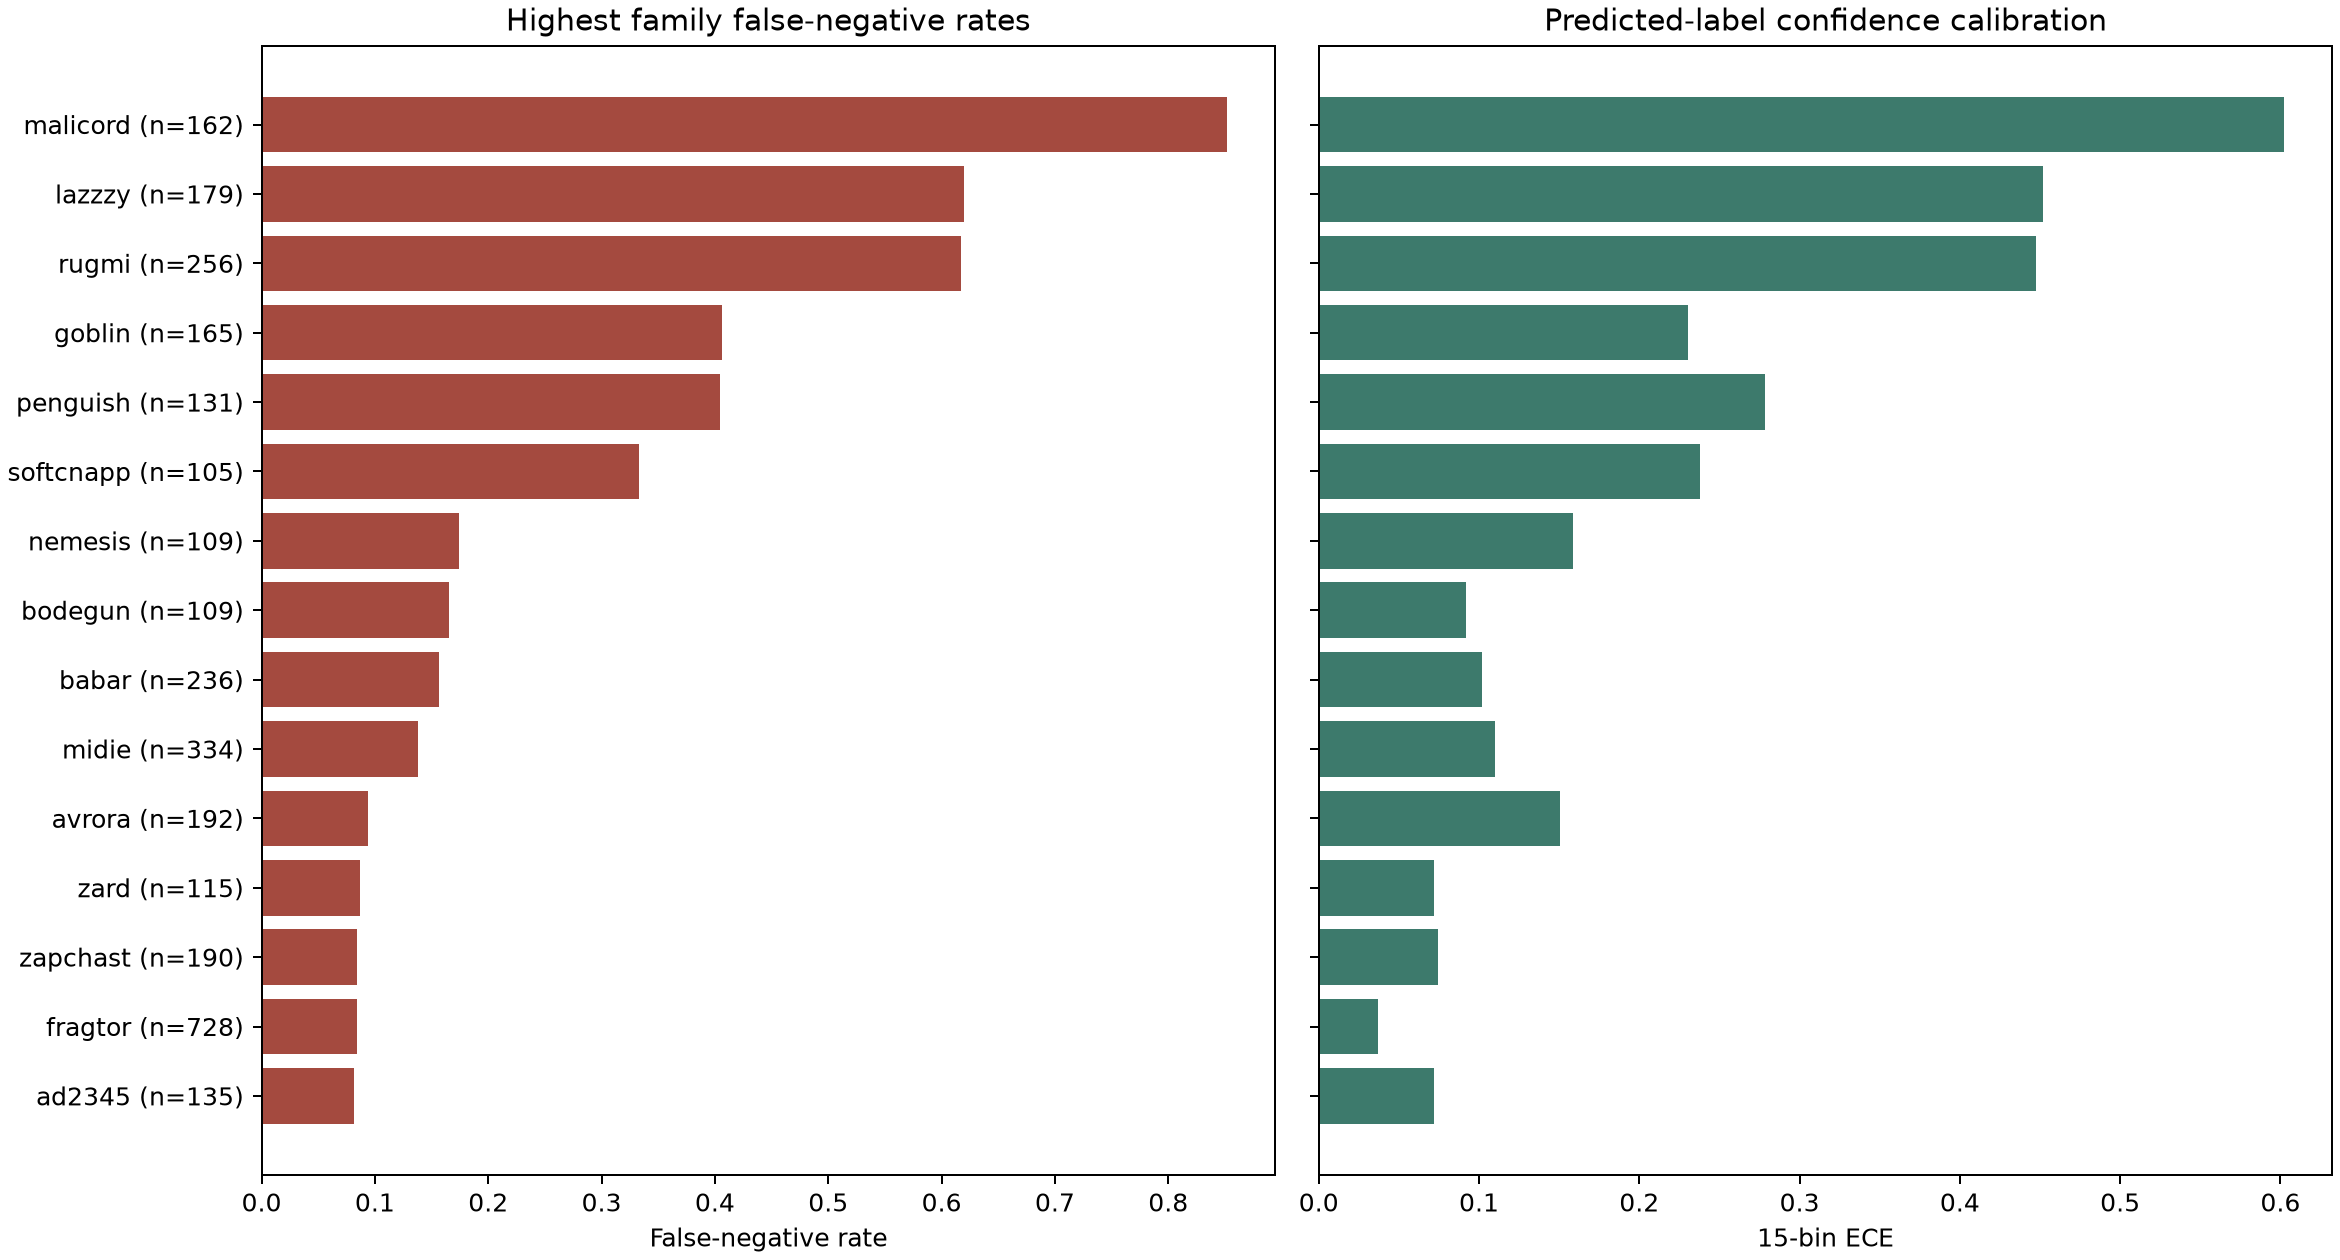
\includegraphics[width=0.92\textwidth]{../results/family_failures.png}
\caption{Largest family false-negative rates and calibration errors.}
\label{fig:family}
\end{figure}

\section{Sensitivity Checks}

\subsection{Calibration bins}

Table~\ref{tab:bins} varies the number of aggregate confidence bins. ECE stays
between 0.00297 and 0.00323. MCE rises as narrower bins expose larger local
gaps. The same ten families appear in the top-ten family-ECE set for every bin
count.

\begin{table}[!htbp]
\centering
\caption{Sensitivity to the number of confidence bins.}
\label{tab:bins}
\begin{tabular}{rrrr}
\toprule
Bins & Aggregate ECE & Aggregate MCE & Family-ECE overlap \\
\midrule
10 & 0.002967793 & 0.023373977 & 10/10 \\
15 & 0.003085084 & 0.027724607 & 10/10 \\
20 & 0.003177991 & 0.029541059 & 10/10 \\
30 & 0.003227550 & 0.035004511 & 10/10 \\
\bottomrule
\end{tabular}
\end{table}

\subsection{Family minimum}

Changing the minimum family size changes both eligibility and the leading
families. Table~\ref{tab:minimum} compares each setting with the primary
100-record top ten. The 50-record rule admits 394 families. Only six of its top
ten false-negative-rate families match the primary list. The 200-record rule
admits 128 families, with only three matches. Small-family rankings should not
be read as precise population estimates.

\begin{table}[!htbp]
\centering
\caption{Sensitivity to the minimum malicious family count.}
\label{tab:minimum}
\begin{tabular}{rrrrr}
\toprule
Minimum & Families & Rows & FNR overlap & ECE overlap \\
\midrule
50 & 394 & 210,067 & 6/10 & 6/10 \\
100 & 232 & 198,854 & 10/10 & 10/10 \\
200 & 128 & 184,149 & 3/10 & 3/10 \\
\bottomrule
\end{tabular}
\end{table}

\section{Limits}

This study has several limits:

\begin{itemize}
  \item Family results are descriptive and do not establish a causal effect.
  \item Many malicious records have no family label. Family labels also come
  from the upstream data and may contain noise.
  \item Estimates for small families are unstable. The study reports no
  confidence intervals.
  \item Sixty hashes repeat across weeks. They have no observed conflicts, but
  a unique-hash sensitivity analysis was not run.
  \item The first structural half was selected by a fixed rule. The study does
  not claim that it is better than the second half.
  \item The evaluation covers PE records and one released model. It does not
  measure other EMBER2024 file types or models.
\end{itemize}

A separate SHAP pipeline used EMBER2018 malicious samples and a separately
trained Random Forest. It therefore did not explain the evaluated EMBER2024
model. SHAP is a method for assigning feature contributions to predictions
\cite{lundberg2017shap}. Model-aligned SHAP, retraining, and post-hoc calibration
are not part of this study.

\section{Reproducibility}

The workflow pins the official source, dataset, and model repository. The exact
identifiers are:

\begin{quote}
\small
Source revision: \code{0ef753e81d98bf209f71b03cd331dfc190b5b54d}\\
Dataset revision: \code{3d23efef7c0f0b702c5024400cfff4c3744a3832}\\
Model revision: \code{e5b945dd90e1a1a1ec0cc07b3a17b52e9ba2d0c2}\\
Model SHA-256: \code{4252027863492ac138785c8c18576f43dad77d00faddc14e8c0072e8db419f99}
\end{quote}

Downloaded files were checked before extraction. The selection manifest records
every selected file and the repeated-hash profile. The preparation manifest
records the row count, order, data types, feature count, sizes, and checksums.
The inference manifest links the released model to the prepared inputs and
predictions. The analysis manifest links those inputs to the small tracked
tables and figures. The analysis code commit is
\code{c63e5548d6c1eab93e57b99e292d1af68fa31318}.

The environment record describes a macOS arm64 Python 3.12 setup with LightGBM
4.7.0, \code{thrember} 0.1.0, and the Homebrew OpenMP runtime. The requirements
snapshot is host-specific, not a universal cross-platform lock file. Synthetic
tests cover archive checks, selection, preparation, inference, and metric
definitions without requiring the large artifacts.

\section{Conclusion}

The released EMBER2024 PE model performs well on the full 540,000-record
evaluation. Its accuracy is 98.03\%, ROC AUC is 0.9982, and 15-bin ECE is
0.0031. These values do not describe every malware family. Several eligible
families have false-negative rates above 0.40, and three are above 0.61.

The evidence supports a limited conclusion. Strong aggregate calibration can
hide large family-level errors. These results identify groups for closer study,
but they do not explain why the errors occur.

\begin{thebibliography}{9}

\bibitem{joyce2025ember}
Robert J. Joyce, Gideon Miller, Phil Roth, Richard Zak, Elliott
Zaresky-Williams, Hyrum Anderson, Edward Raff, and James Holt.
\newblock EMBER2024 - A Benchmark Dataset for Holistic Evaluation of Malware
Classifiers.
\newblock Proceedings of the 31st ACM SIGKDD Conference on Knowledge Discovery
and Data Mining, 2025.
\newblock \url{https://arxiv.org/abs/2506.05074}.

\bibitem{ke2017lightgbm}
Guolin Ke, Qi Meng, Thomas Finley, Taifeng Wang, Wei Chen, Weidong Ma, Qiwei Ye,
and Tie-Yan Liu.
\newblock LightGBM: A Highly Efficient Gradient Boosting Decision Tree.
\newblock Advances in Neural Information Processing Systems 30, 2017.
\newblock \url{https://proceedings.neurips.cc/paper/2017/hash/6449f44a102fde848669bdd9eb6b76fa-Abstract.html}.

\bibitem{brier1950}
Glenn W. Brier.
\newblock Verification of Forecasts Expressed in Terms of Probability.
\newblock Monthly Weather Review, 78(1):1--3, 1950.
\newblock \url{https://doi.org/10.1175/1520-0493(1950)078<0001:VOFEIT>2.0.CO;2}.

\bibitem{guo2017calibration}
Chuan Guo, Geoff Pleiss, Yu Sun, and Kilian Q. Weinberger.
\newblock On Calibration of Modern Neural Networks.
\newblock Proceedings of the 34th International Conference on Machine Learning,
70:1321--1330, 2017.
\newblock \url{https://proceedings.mlr.press/v70/guo17a.html}.

\bibitem{lundberg2017shap}
Scott M. Lundberg and Su-In Lee.
\newblock A Unified Approach to Interpreting Model Predictions.
\newblock Advances in Neural Information Processing Systems 30, 2017.
\newblock \url{https://proceedings.neurips.cc/paper/2017/hash/8a20a8621978632d76c43dfd28b67767-Abstract.html}.

\end{thebibliography}

\end{document}
